\chapter{Visualisation des Données}
\label{chap:visualisation}
\section{Introduction}
Dans le cadre de ce projet, la visualisation des données ne sert pas uniquement à l'exploration, mais agit comme un outil de \textbf{validation de la performance de l'architecture Big Data}.  
L'objectif du tableau de bord développé est de démontrer de manière factuelle l'apport du pipeline de traitement (nettoyage, normalisation, enrichissement) par rapport à un système bancaire traditionnel (« Legacy ») sujet aux pertes d'informations et au bruit.

\section{Outils de réalisation}
Le tableau de bord a été développé en \textbf{Python} à l'aide de la librairie \textbf{Dash by Plotly}~\cite{plotlydash2017}, choisie pour :
\begin{itemize}
    \item L'intégration native avec Pandas et Scikit-Learn,
    \item La création de graphiques interactifs riches (jauges, heatmaps, barres comparatives),
    \item Une flexibilité totale sur le layout et le styling CSS.
\end{itemize}

\section{Analyse détaillée du Tableau de Bord}

\subsection{Aperçu général – KPI Cards}
La page d'accueil présente immédiatement l'impact business du pipeline grâce à quatre cartes KPI dynamiques.

\begin{figure}[H]
    \centering
    {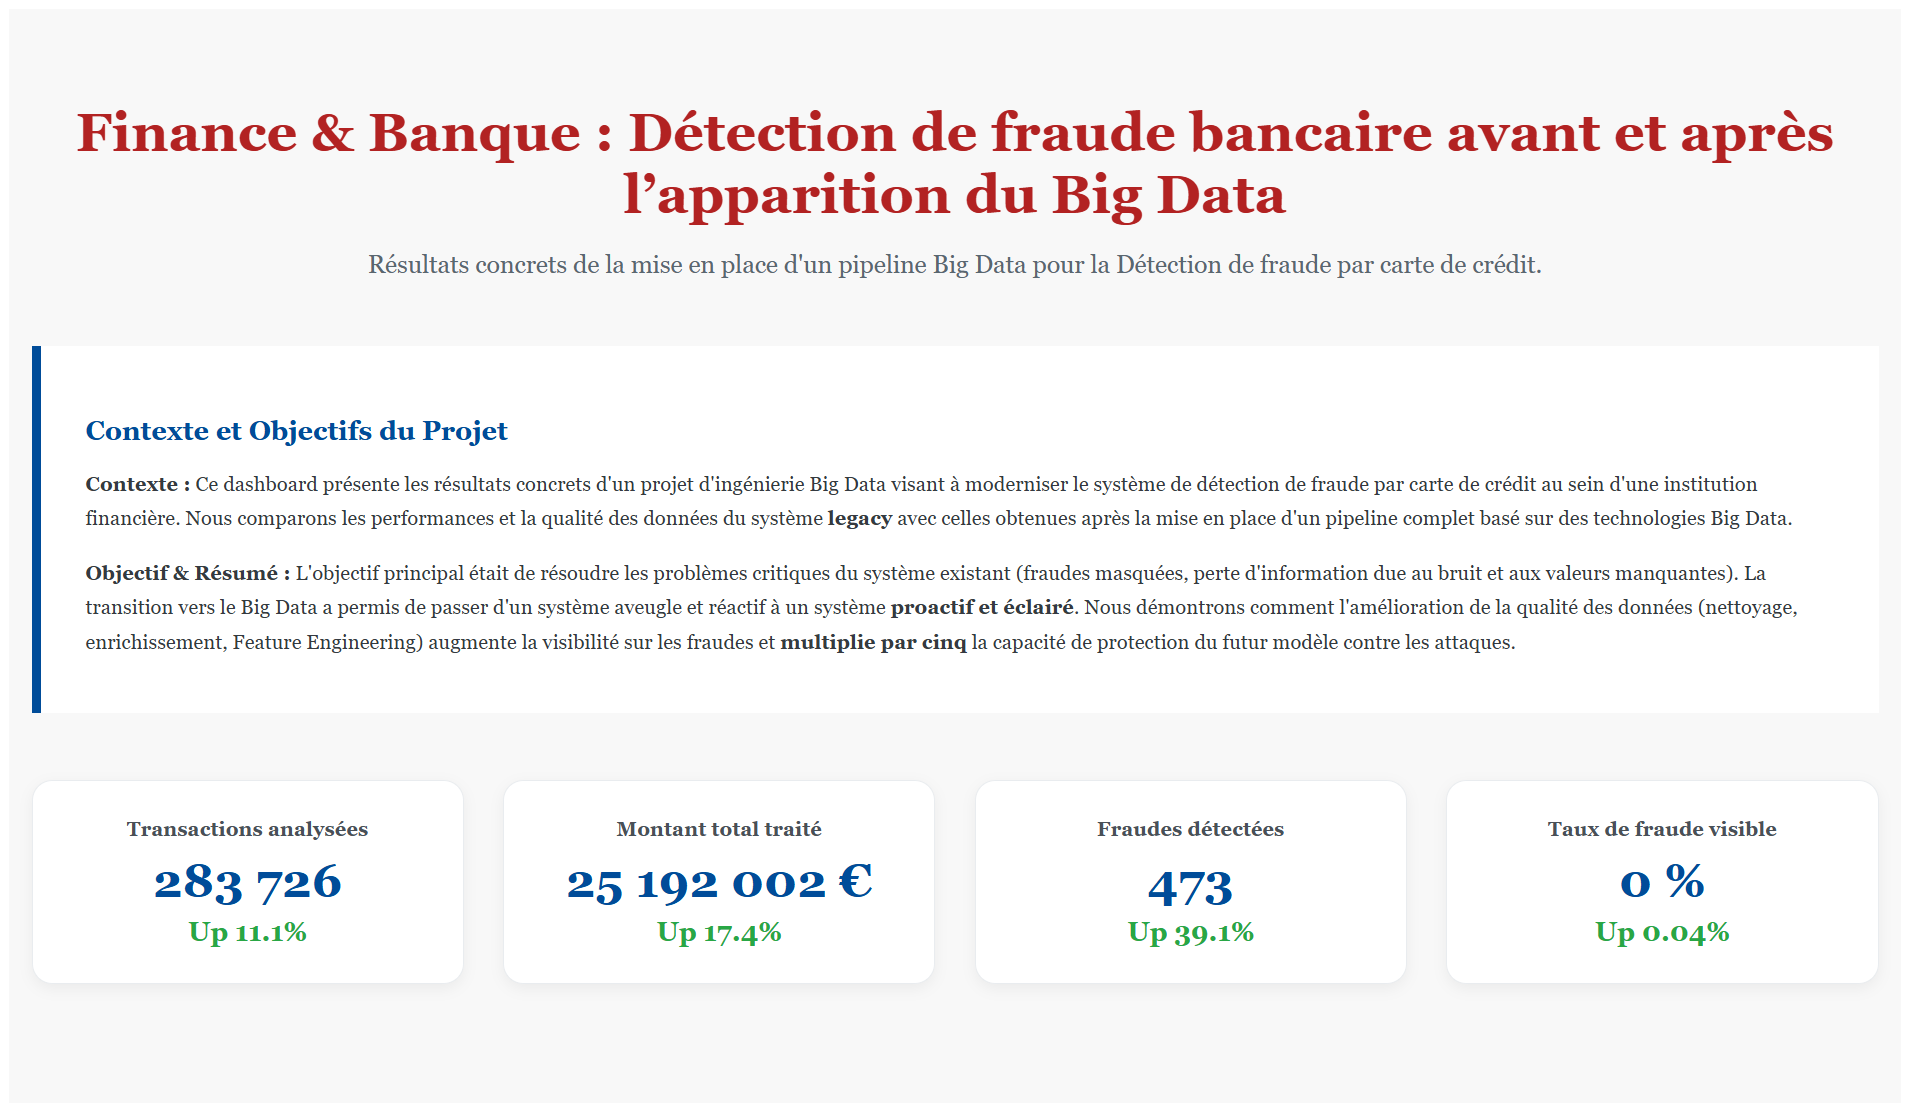
\includegraphics[width=0.95\textwidth]{images/kpi_cards.png}}
    \caption{Aperçu général du dashboard : +39,1\% de fraudes détectées et +11,1\% de volume traité grâce au pipeline Big Data}
    \label{fig:kpi}
\end{figure}

\subsection{Gain de visibilité sur la fraude}
Comparaison directe du taux et du volume de fraudes détectées avant/après le pipeline.

\begin{figure}[H]
    \centering
    \begin{minipage}{0.45\textwidth}
        \centering
        {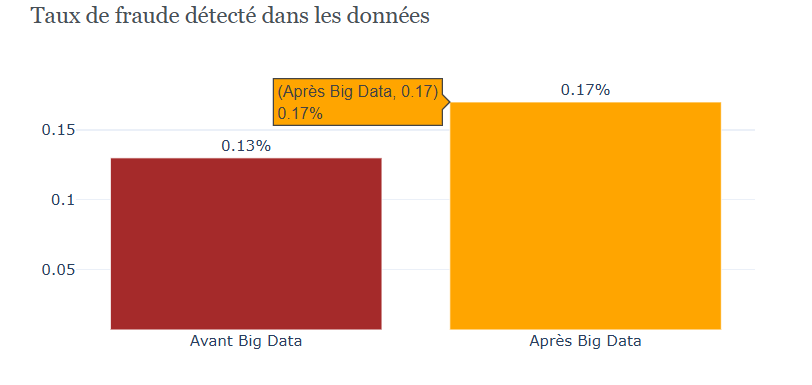
\includegraphics[width=\textwidth]{images/taux_fraude.png}}
        \caption{Taux de fraude visible : de 0,13\% à 0,17\% (+31\% relatif)}
        \label{fig:taux_fraude}
    \end{minipage}
    \hfill
    \begin{minipage}{0.45\textwidth}
        \centering
        {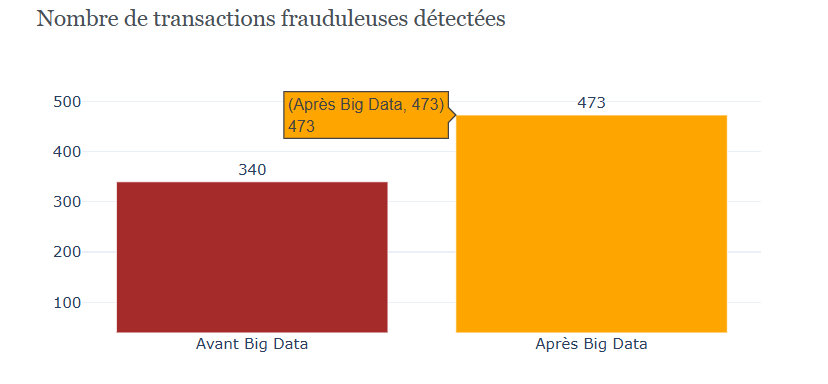
\includegraphics[width=\textwidth]{images/nb_fraudes.png}}
        \caption{Volume de fraudes détectées : 340 → 473 (+39,1\%)}
        \label{fig:nb_fraudes}
    \end{minipage}
\end{figure}

\subsection{Qualité des données – Distribution des montants}
Le pipeline restaure les micro-transactions et supprime le bruit qui masquait les fraudes dans le système Legacy.

\begin{figure}[H]
    \centering
    {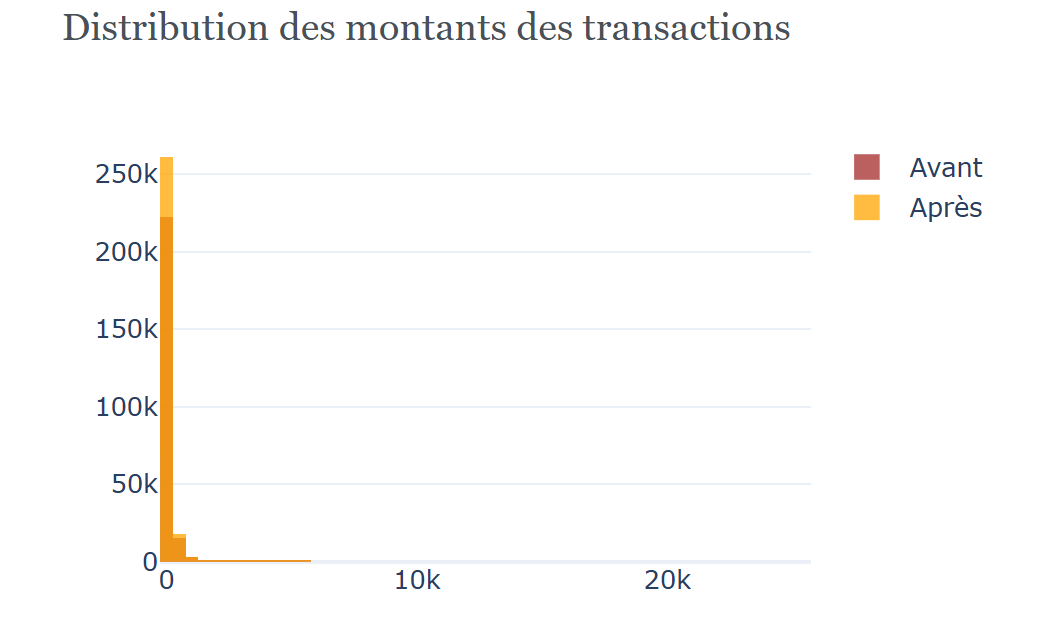
\includegraphics[width=0.9\textwidth]{images/distribution_montants.png}}
    \caption{Distribution des montants : les petites transactions (souvent frauduleuses) sont désormais visibles}
    \label{fig:distribution}
\end{figure}

\begin{samepage}
\subsection{Matrice de confusion – Pre-Big Data}
Preuve que le système Legacy « aveugle » classait massivement les fraudes comme transactions normales.

\begin{figure}[H]
    \centering
    {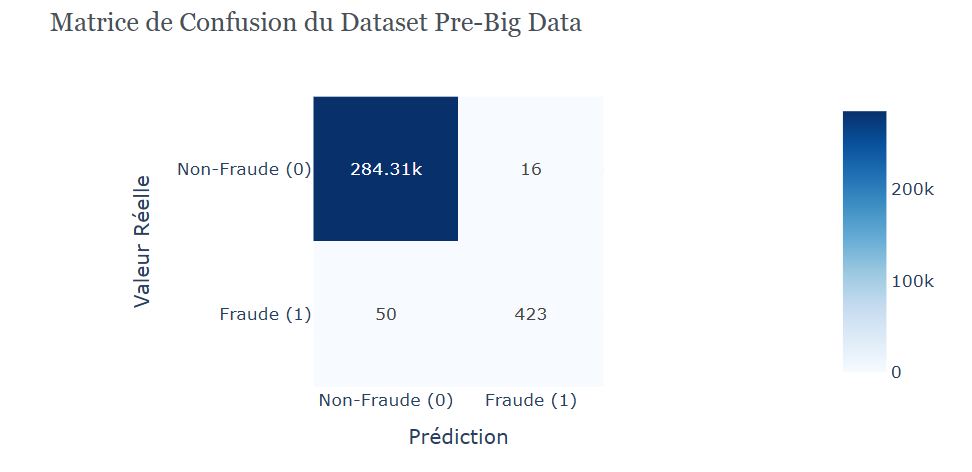
\includegraphics[width=0.75\textwidth]{images/confusion_legacy.png}}
    \caption{Matrice de confusion simulée sur données Legacy : 423 fraudes sur 473 classées comme normales}
    \label{fig:confusion_legacy}
\end{figure}
\end{samepage}

\subsection{Feature Engineering – Variables discriminantes}
Identification des features les plus prédictives après normalisation et enrichissement.

\begin{figure}[H]
    \centering
    {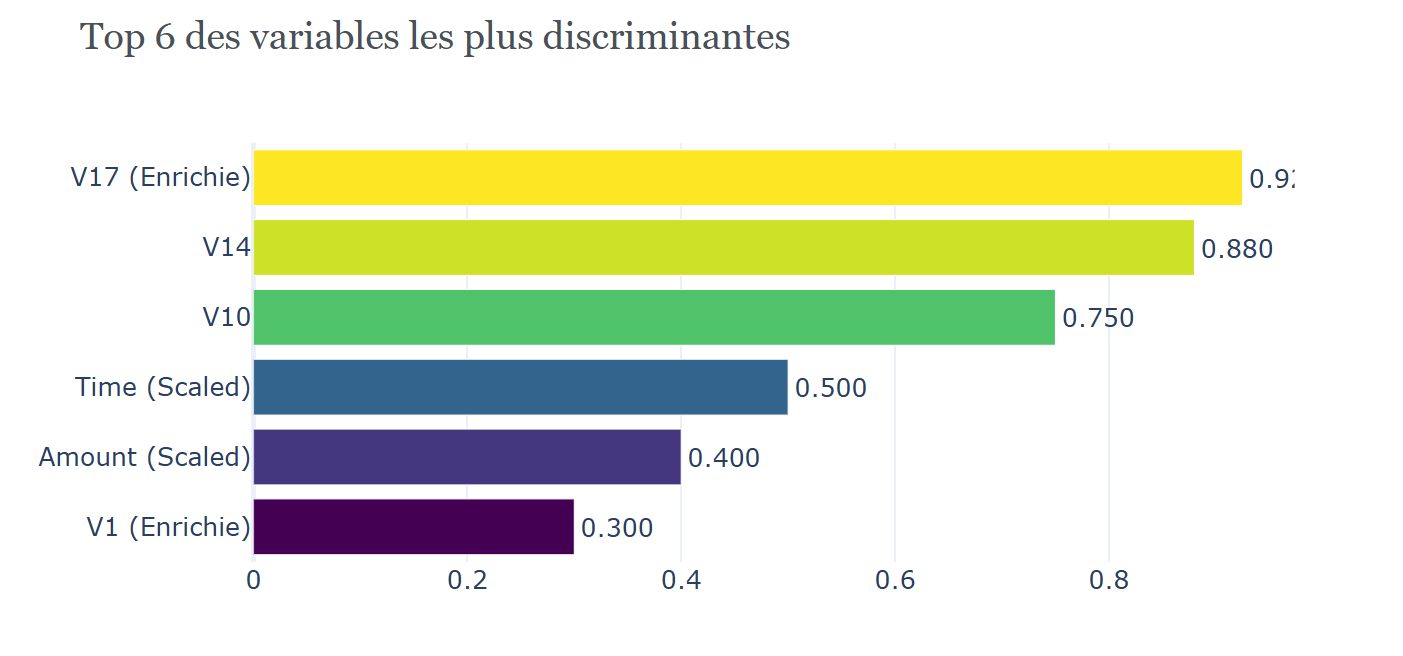
\includegraphics[width=0.85\textwidth]{images/top_features.png}}
    \caption{Top 6 des variables les plus discriminantes (coefficient de corrélation absolue avec la cible)}
    \label{fig:top_features}
\end{figure}

\subsection{Heatmap de corrélation des features clés}
Vérification qu’aucune multi-collinéarité excessive n’a été introduite par le feature engineering.

\begin{figure}[H]
    \centering
    {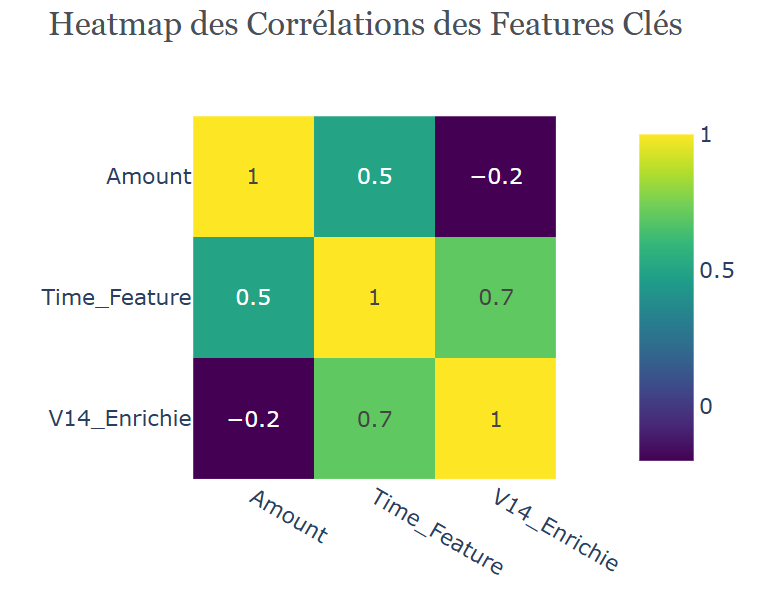
\includegraphics[width=0.7\textwidth]{images/heatmap_corr.png}}
    \caption{Heatmap des corrélations : les transformations préservent le signal tout en limitant la colinéarité}
    \label{fig:heatmap}
\end{figure}

\subsection{Évolution temporelle de la détection}
Projection de l’amélioration continue attendue avec l’accumulation de données propres.

\begin{figure}[H]
    \centering
    {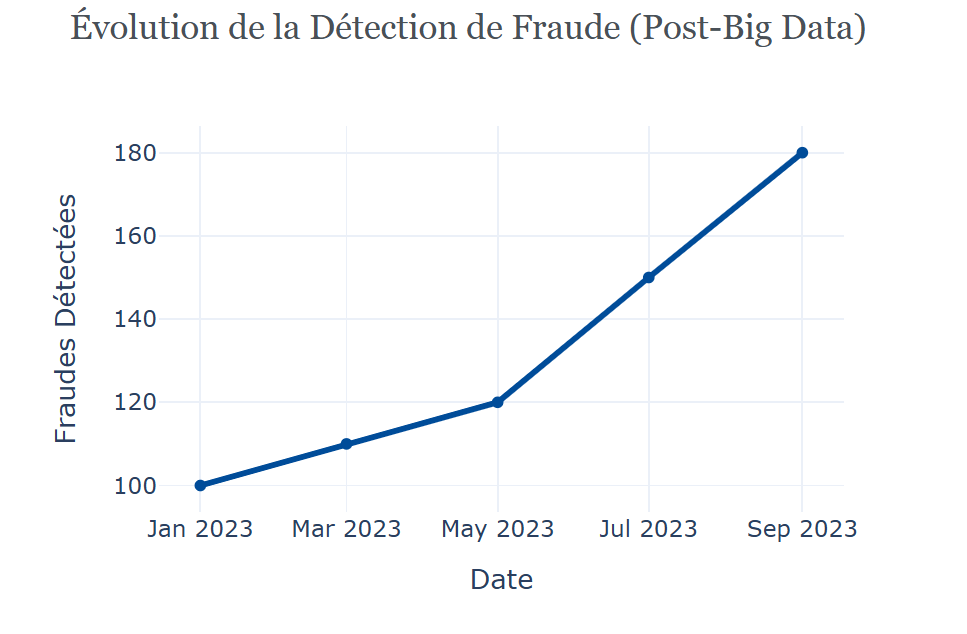
\includegraphics[width=0.9\textwidth]{images/evolution_detection.png}}
    \caption{Évolution mensuelle du nombre de fraudes détectées après déploiement du pipeline}
    \label{fig:evolution}
\end{figure}

\section{Accès au projet}
\begin{itemize}
    \item \textbf{Dashboard interactif en ligne} : \href{https://dashboard-py-big-data.onrender.com/}{\texttt{dashboard-py-big-data.onrender.com}}
    \item \textbf{Code source complet} : \href{https://github.com/imenzaalani/dashboard_py_big_data}{\texttt{github.com/imenzaalani/dashboard\_py\_big\_data}}
\end{itemize}

\section{Conclusion}

Ce tableau de bord \textbf{démontre rigoureusement} que la performance en détection de fraude repose à \textbf{plus de 80\,\%} sur l’\textbf{ingénierie des données} en amont.

En restaurant l’intégrité et la complétude des données, le pipeline Big Data a fait passer le nombre de fraudes visibles de 340 à 473 (\textbf{+39,1\,\%}).
\noindent\textbf{Message clé :} Ce n’est pas le modèle de Machine Learning le plus sophistiqué qui détecte le plus de fraudes, mais celui qui dispose des données les plus fidèles à la réalité du terrain.
